\documentclass[border=4pt]{standalone}
\usepackage{tikz}
\usepackage{xcolor}
\usetikzlibrary{arrows.meta, positioning}
\newcommand{\pillar}[1]{\textcolor{blue!55!black}{\footnotesize\itshape #1}}
\begin{document}
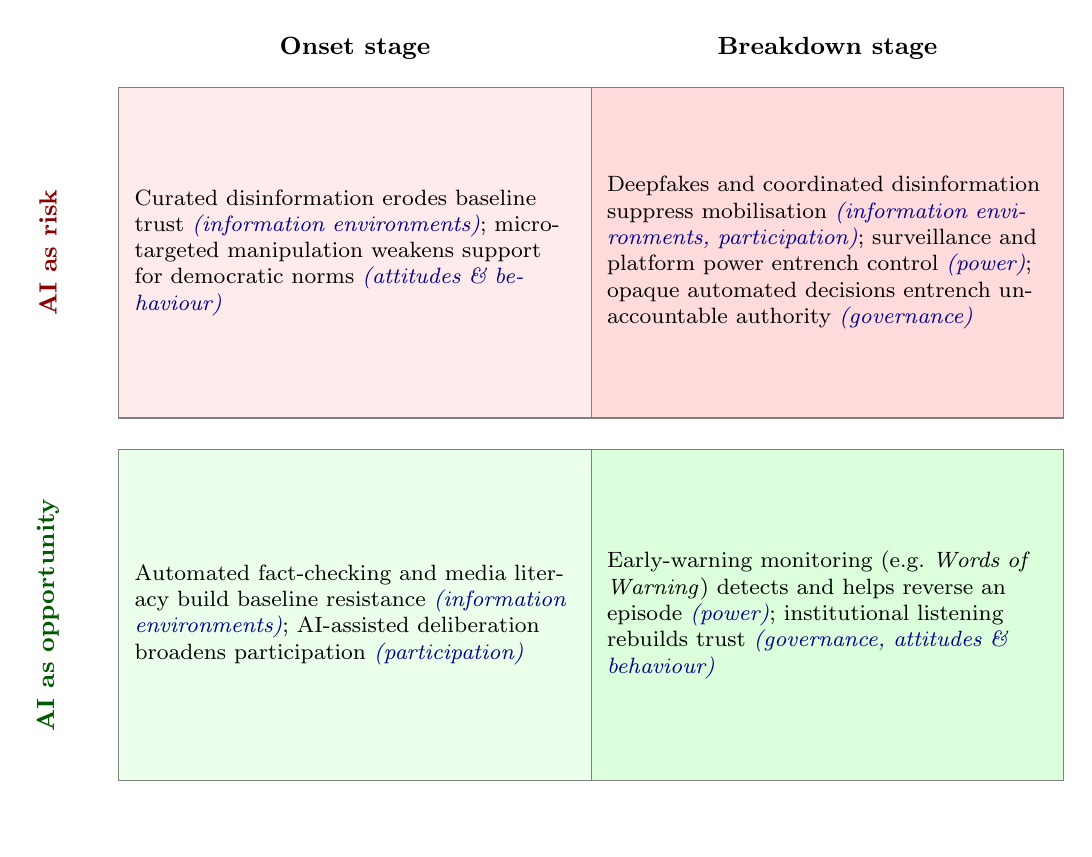
\begin{tikzpicture}[
  every node/.style = {font=\small},
  axislabel/.style = {font=\bfseries\small, align=center},
  celltext/.style = {font=\footnotesize, align=left, text width=5.6cm},
  pillar/.style = {font=\scriptsize\itshape},
  rowlabel/.style = {font=\bfseries\small, align=center, rotate=90},
  >=Latex
]
  \fill[red!8]  (0,0) rectangle (6,4.2);
  \fill[red!14] (6,0) rectangle (12,4.2);
  \fill[green!8] (0,-4.6) rectangle (6,-0.4);
  \fill[green!14] (6,-4.6) rectangle (12,-0.4);
  \draw[gray] (0,0) rectangle (12,4.2);
  \draw[gray] (0,-4.6) rectangle (12,-0.4);
  \draw[gray] (6,0) -- (6,4.2);
  \draw[gray] (6,-4.6) -- (6,-0.4);

  \node[axislabel] at (3,4.7) {Onset stage};
  \node[axislabel] at (9,4.7) {Breakdown stage};
  \node[font=\scriptsize, align=center, text width=5.6cm] at (3,-5.1) {};
  \node[font=\scriptsize, align=center, text width=5.6cm] at (9,-5.1) {};

  \node[rowlabel, red!55!black] at (-0.9,2.1) {AI as risk};
  \node[rowlabel, green!35!black] at (-0.9,-2.5) {AI as opportunity};

  \node[celltext] at (3,2.1) {Curated disinformation erodes baseline trust \pillar{(information environments)}; micro-targeted manipulation weakens support for democratic norms \pillar{(attitudes \& behaviour)}};

  \node[celltext] at (9,2.1) {Deepfakes and coordinated disinformation suppress mobilisation \pillar{(information environments, participation)}; surveillance and platform power entrench control \pillar{(power)}; opaque automated decisions entrench unaccountable authority \pillar{(governance)}};

  \node[celltext] at (3,-2.5) {Automated fact-checking and media literacy build baseline resistance \pillar{(information environments)}; AI-assisted deliberation broadens participation \pillar{(participation)}};

  \node[celltext] at (9,-2.5) {Early-warning monitoring (e.g.\ \emph{Words of Warning}) detects and helps reverse an episode \pillar{(power)}; institutional listening rebuilds trust \pillar{(governance, attitudes \& behaviour)}};
\end{tikzpicture}
\end{document}
